%% graph G_1
\subfigure[$G_1$]{
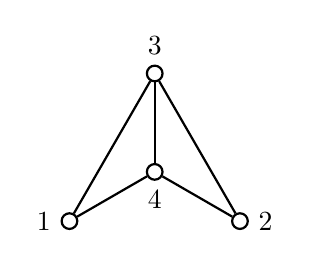
\begin{tikzpicture}
[nodedecorate/.style={shape=circle,inner sep=2pt,draw,thick},%
  linedecorate/.style={-,thick},%
  scale=1.25]
%% nodes or vertices
\foreach \nodename/\x/\y/\direction/\navigate in {
  1/-0.8660/-0.5/left/west, 2/0.8660/-0.5/right/east,
  3/0/1/above/north, 4/0/0/below/south}
{
  \node (\nodename) at (\x,\y) [nodedecorate] {};
  \node [\direction] at (\nodename.\navigate) {$\nodename$};
}
%% edges or lines
\path
\foreach \startnode/\endnode in {1/3, 1/4, 2/3, 2/4, 3/4} {
  (\startnode) edge[linedecorate] node {} (\endnode)
};
\end{tikzpicture}
}
%%
%% graph G_2
\subfigure[$G_2$]{
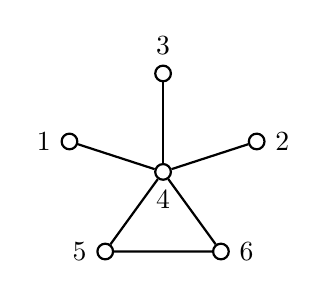
\begin{tikzpicture}
[nodedecorate/.style={shape=circle,inner sep=2pt,draw,thick},%
  linedecorate/.style={-,thick},%
  scale=1.25]
%% nodes or vertices
\foreach \nodename/\x/\y/\direction/\navigate in {
  1/-0.9510/0.3090/left/west, 2/0.9510/0.3090/right/east,
  3/0/1/above/north, 4/0/0/below/south, 5/-0.5877/-0.8090/left/west,
  6/0.5877/-0.8090/right/east}
{
  \node (\nodename) at (\x,\y) [nodedecorate] {};
  \node [\direction] at (\nodename.\navigate) {$\nodename$};
}
%% edges or lines
\path
\foreach \startnode/\endnode in {1/4, 2/4, 3/4, 4/5, 4/6, 5/6} {
  (\startnode) edge[linedecorate] node {} (\endnode)
};
\end{tikzpicture}
}
%%
%% graph G_1 union G_2
\subfigure[$G_1 \cup G_2$]{
\label{fig:introduction:union_graphs_overlapping_vertex_sets}
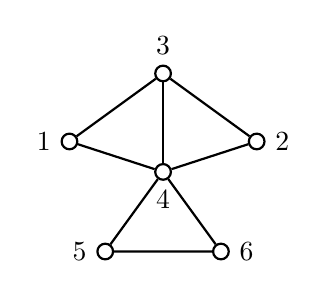
\begin{tikzpicture}
[nodedecorate/.style={shape=circle,inner sep=2pt,draw,thick},%
  linedecorate/.style={-,thick},%
  scale=1.25]
%% nodes or vertices
\foreach \nodename/\x/\y/\direction/\navigate in {
  1/-0.9510/0.3090/left/west, 2/0.9510/0.3090/right/east,
  3/0/1/above/north, 4/0/0/below/south, 5/-0.5877/-0.8090/left/west,
  6/0.5877/-0.8090/right/east}
{
  \node (\nodename) at (\x,\y) [nodedecorate] {};
  \node [\direction] at (\nodename.\navigate) {$\nodename$};
}
%% edges or lines
\path
\foreach \startnode/\endnode in {1/4, 1/3, 2/3, 2/4, 3/4, 4/5, 4/6, 5/6} {
  (\startnode) edge[linedecorate] node {} (\endnode)
};
\end{tikzpicture}
}
%%
%% graph G_1 intersect G_2
\subfigure[$G_1 \cap G_2$]{
\label{fig:introduction:intersection_graphs_overlapping_vertex_sets}
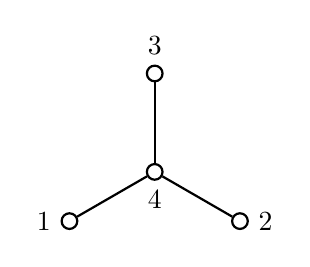
\begin{tikzpicture}
[nodedecorate/.style={shape=circle,inner sep=2pt,draw,thick},%
  linedecorate/.style={-,thick},%
  scale=1.25]
%% nodes or vertices
\foreach \nodename/\x/\y/\direction/\navigate in {
  1/-0.8660/-0.5/left/west, 2/0.8660/-0.5/right/east,
  3/0/1/above/north, 4/0/0/below/south}
{
  \node (\nodename) at (\x,\y) [nodedecorate] {};
  \node [\direction] at (\nodename.\navigate) {$\nodename$};
}
%% edges or lines
\path
\foreach \startnode/\endnode in {1/4, 2/4, 3/4} {
  (\startnode) edge[linedecorate] node {} (\endnode)
};
\end{tikzpicture}
}
